\section{Proceso Puntual}

Un proceso puntual es un proceso estocástico que es utilizado para modelar eventos que ocurren en intervalos aleatorios y relativos al eje del tiempo o del espacio. Estos, describen un subconjunto aleatorio de puntos en algún espacio $\mathcal{X}$ o la ocurrencia a lo largo del tiempo de eventos aleatorios secuenciales. 

\vspace{0.2cm}

Si bien existe una definición más general de un proceso puntual, nos centraremos en el caso particular discreto y real. Sea $\mathcal{Y}$ un conjunto de puntos de la forma $\{ 1 , \dots , N \}$ y denotemos $N(\mathcal{Y})$ como el conjunto de todas las medidas puntuales sobre $\mathcal{Y}$. Se dirá que $\mathcal{P}$ es un proceso puntual sobre $\mathcal{Y}$ si es una medida de probabilidad sobre $N(\mathcal{Y})$ y lo denotaremos como $Y \sim PP(\mathcal{Y})$. 

\vspace{0.2cm}

Existen múltiples procesos puntuales entre los que podemos destacar los procesos de \textit{Poisson}, \textit{Markov Random Fields}, procesos de \textit{Cox}, entre otros. 


\subsection{Procesos Puntuales Determinantales}

Los Procesos Puntuales Determinantales, desde ahora DPP, son modelos probabilísticos de repulsión (procesos repulsivos) que surgen naturalmente en mecánica cuántica y en teoría de matrices aleatorias y que, a diferencia de otros modelos utilizados como \textit{Markov Random Fields}, estos proveen algoritmos eficientes y exactos para samplear, marginalizar, condicionar, entre otras tareas de inferencia \cite{Kulesza_2012}.


\subsubsection{Definición }

De manera formal, un DPP es un proceso puntual estocástico cuya distribución de probabilidad queda completamente definida por el determinante de alguna función. En particular si $Y \sim PP(\mathcal{Y})$ acorde a $\mathcal{P}$ tal que 
\[ (\forall A \subseteq \mathcal{Y}): \mathcal{P}(A \subseteq Y) = \det(K_A) ,  \]
entonces diremos que $Y \sim DPP(\mathcal{Y})$. Aquí, $K_A$ es la restricción a las columnas definidas por el conjunto $A$ de una matriz $K \in \mathcal{M}_{N \times N} (\mathbb{R})$ definida positiva, simétrica y a valores propios acotados por 1 cuya indexación está definida por $\mathcal{Y}$ y se le conoce como kernel marginal. Una observación sencilla es que si $A = \{i\}$ un singleton, entonces 
\[ \mathcal{P}(i \in Y) = K_{ii} ,  \]
y por tanto, las diagonales con números cercanos a 1 corresponden a elementos que pueden ser seleccionados con alta probabilidad. Por otro lado, si $A = \{i,j\}$, entonces
	\[
	\mathcal{P}(i,j \in Y) = \begin{vmatrix}
    K_{ii} & K_{ij} \\ 
    K_{ji} & K_{jj}
    \end{vmatrix} = K_{ii}K_{jj} - K_{ji}K_{ij} = \mathcal{P}(i \in Y)\mathcal{P}(j \in Y) - K_{ij}^2 , 
	\] es decir, los elementos fuera de la diagonal representan correlaciones entre pares de elementos, entre mayor sea el valor de $K_{ij}^2$, menor será la probabilidad de que $i,j$ aparezcan juntos. Finalmente, dado que $K$ debe ser una matriz definida positiva, es posible probar que $K_{ij}^2 \leq K_{ii}K_{jj}$ y por tanto, lo anterior logra definir una probabilidad. 
%es decir, los elementos fuera de la diagonal corresponden a las correlaciones negativas entre pares de elementos.

\subsubsection{Aplicaciones }

Existen numerosos casos de uso de los DPP, se mencionan algunos de ellos a continuación: 

\begin{itemize}
    \item \textbf{Valores propios de Matrices Aleatorias} \cite{MEHTA1960420}\cite{doi:10.1063/1.1704292}
    
    Sea $M$ una matriz aleatoria tomando cada entrada independientemente de una distribución normal compleja. 

    Los valores propios de $M$ que forman un subconjunto del plano complejo, están distribuidos acorde a un DPP. 
    
    \item \textbf{Random Walks No-Intersectantes} \cite{Johansson_2004} 
    
    Consideremos un conjunto de $k$ caminatas aleatorias simples, independientes, enteras, de largo $T$. Si comienzan de  $x_{1}^{1} , x_{1}^{2} , \dots , x_{1}^{k}$, condicionadas a que no se intersecten y terminen en $x_{T}^{1} , x_{T}^{2} , \dots , x_{T}^{k}$. Entonces para cada instante $t$, $x_{t}^{1} , x_{t}^{2} , \dots , x_{t}^{k}$ distribuye como un DPP.
    
    \item \textbf{Aristas de Spanning Trees Aleatorios. }\cite{https://doi.org/10.48550/arxiv.math/0404048}
    
    Sea $G$ un grafo arbitrario finito con $N$ aristas y sea $T$ un árbol generador escogido aleatoriamente del conjunto de todos los árboles generadores de $G$. Las aristas de $T$ que forman un subconjunto de $T$ distribuyen como un DPP.  
    
    \item \textbf{Descensos en Secuencias Aleatorias. } \cite{https://doi.org/10.48550/arxiv.0904.3740}

    Dada una secuencia de $N$ números escogidos de forma independiente y uniforme de un conjunto finito de números (del 1 al 9 por ejemplo), la posición en la secuencia donde tal número es menor que el escogido previamente forma un subconjunto de \{2 , \dots , N\} y distribuye como un DPP.
    
\end{itemize}

\subsubsection{Sampling}

Antes de definir el algoritmo de sampleo, es útil definir los DPP no a través de su kernel marginal $K$, y más bien por una matriz $L$ que llamamos L-ensamblaje. Sea $Y$ un conjunto dado e $\textbf{Y}$ un conjunto aleatorio, la matriz de L-ensamblaje es tal que 
\[ \mathcal{P}_{L}(\textbf{Y} = Y) \propto \det(L_Y) ,  \]
con $L_Y$ la restricción de $L$ a los índices de $Y$. Lo anterior define de forma atómica la probabilidad de observar el conjunto $Y$. En este caso, es evidente que $L$ debe ser definida semi-positiva (para que pueda definir una probabilidad) pero gracias a que sólo es una relación de proporcionalidad, no es necesario pedir que la matriz tenga valores propios acotados por 1. 

\vspace{0.2cm}

Es posible probar que la constante de proporcionalidad viene dada por $\frac{1}{\det(L + I)}$ con $I$ la matriz identidad con las mismas dimensiones de $L$ (\hyperlink{Teorema B.1}{Teorema B.1}). Por otro lado, obtener la matriz $K$ a través de $L$ es posible mediante la ecuación (\hyperlink{Teorema B.2}{Teorema B.2})
\[
K = L(L+I)^{-1} = I - (L+I)^{-1} , 
\]
y de forma inversa, 
\[
L = K(I-K)^{-1} , 
\]
la observación fundamental es que es posible computar $K$ mediante la descomposición en valores y vectores propios de $L = \sum_{n=1}^{N} \lambda_nv_n v^{\top}_n$ simplemente reescalando 
\[
K = \sum_{n=1}^{N}\frac{\lambda_n}{\lambda_n + 1}v_n v^{\top}_n .
\]
Notar que no todo kernel marginal define un $L$-ensamblaje, en particular cuando alguno de sus valores propios alcanza el valor de $1$ pues la matriz $(I-K)$ deja de ser invertible. Estamos en condiciones de definir el algoritmo de sampleo para un DPP.

\begin{teo}
Sea $L = \sum_{n=1}^N \lambda_n v_n v_{n}^{\top}$ una descomposición ortonormal de una matriz semidefinida positiva $L$. El siguiente algoritmo samplea $\mathbf{Y} \sim \mathcal{P}_L$.

\begin{algorithm}
\caption{Muestreo de un DPP $O(Nk^3)$, $k = |V|$ (Kulesza 2012)}\label{alg:alg1}
\begin{algorithmic}
\Require Descomposición en valores y vectores propios 
$\{(v_n , \lambda_n)\}_{n}$ de $L$
\State $J \gets \emptyset$
\For{n = 1 , \dots , N}
\State $J \gets J \cup \{n\}$ con probabilidad $\frac{\lambda_n}{\lambda_n+1}$
\EndFor
\State $V \gets \{ v_n \}_{n \in J}$
\State $Y \gets \emptyset$
\While{$|V| > 0$}
\State Seleccionar $i$ de $\mathcal{Y}$ con probabilidad $Pr(i) = \frac{1}{|V|}\sum_{v \in V}(v^{\top}e_i)^2$ con $e_i$ vector canónico de dimensión $N$                                                                               
\State $Y \gets Y \cup i$
\State $V \gets V_{\perp}$, una base ortonormal del subespacio de $V$ ortogonal a $e_i$ 
\EndWhile   
\State \textbf{Output: } $Y$
\end{algorithmic}
\end{algorithm}
\end{teo}

\begin{figure}[ht]
    \centering
    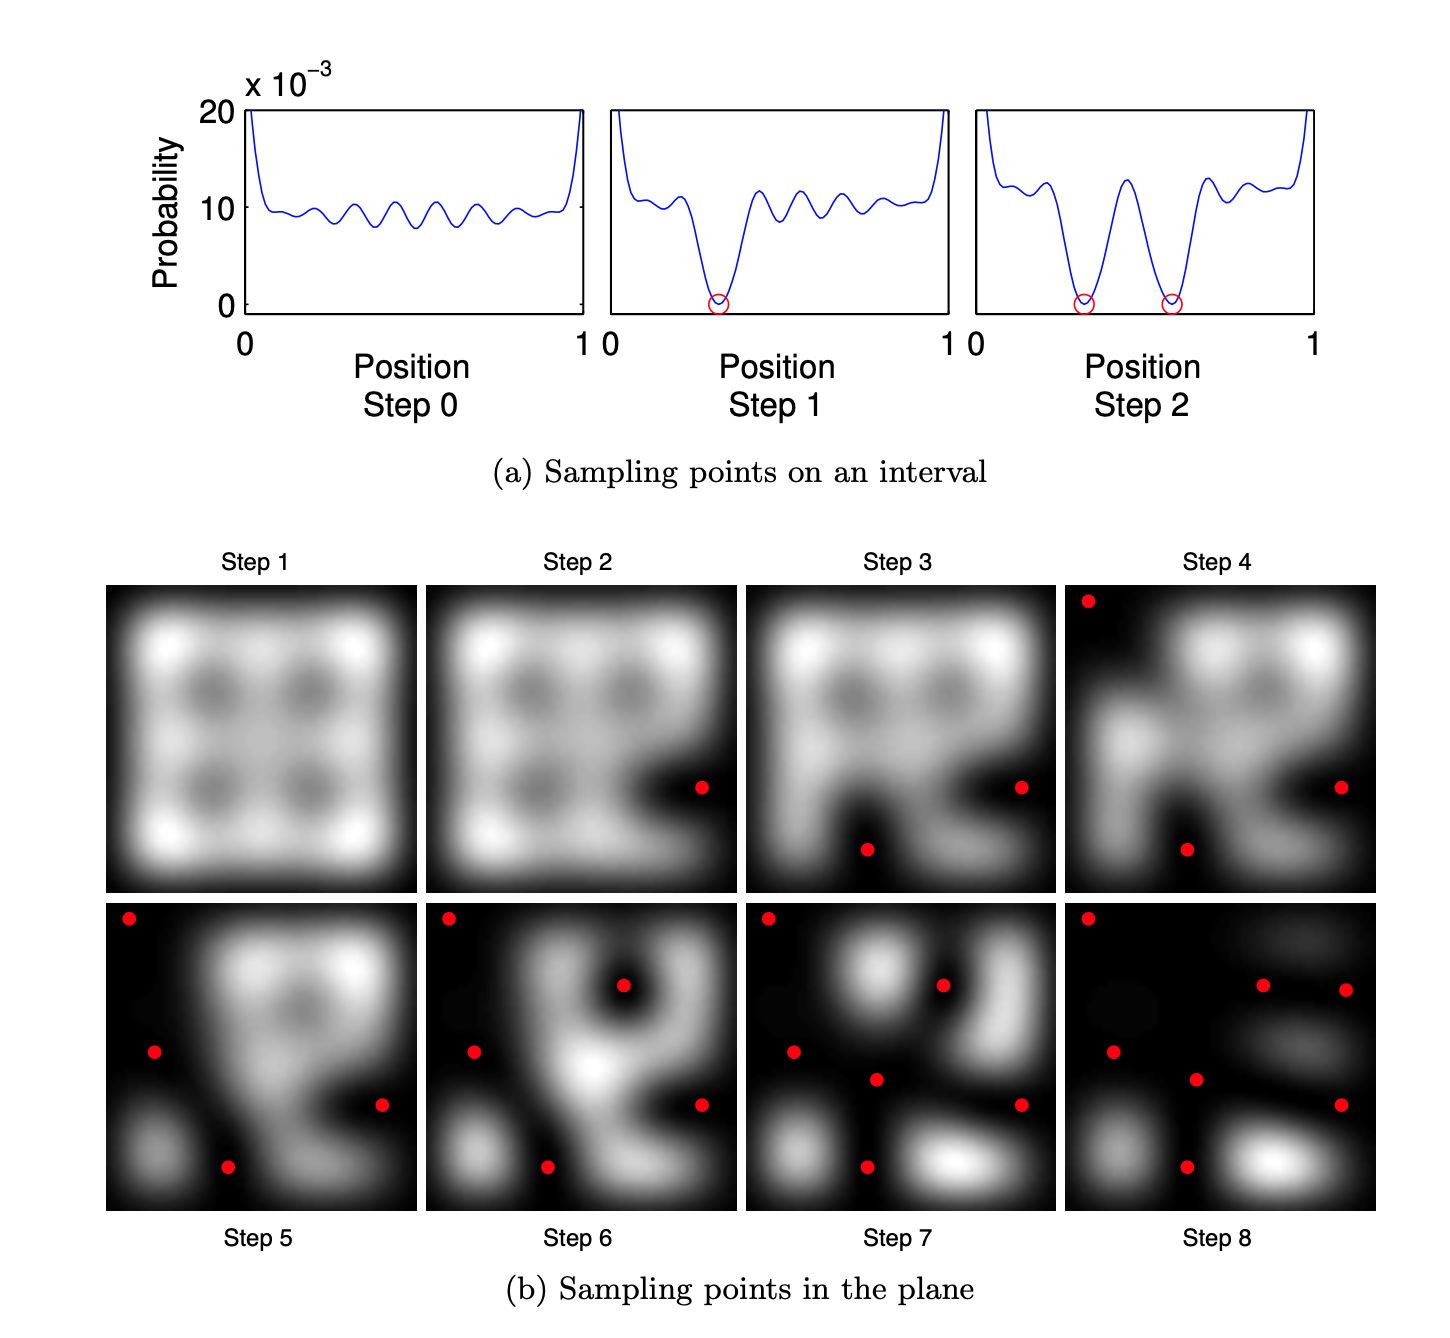
\includegraphics[width=12cm]{img/tesis/DPP_sampling.png}
    \caption{Muestreo de un DPP en una y dos dimensiones. Cada ejemplo sampleado disminuye la probabilidad de muestrear otro en una vecindad cercana (Kulesza 2012)}
    \label{fig:example}
\end{figure}

La demostración de este teorema es extensa y por tanto no incluida en el marco teórico, la complejidad del algoritmo es principalmente causada por la ortonormalización \textit{Gram-Schmidt} $O(Nk^2)$ necesaria para calcular $V_{\perp}$. Por otro lado, existe un algoritmo de sampleo alternativo y más eficiente en situaciones en las que $N$ es grande. 

\vspace{0.2cm}

Sea $L$ un $L$-ensamblaje y consideremos la descomposición de \textit{Cholesky} $L = B^{\top}B$ con $B \in \mathcal{M}_{D \times N}(\mathbb{R})$ donde $D \leq N$, se define 
\[
C = BB^{\top}, 
\]
por lo que $C \in \mathcal{M}_{D \times D}(\mathbb{R})$, es idealmente, una matriz de menor dimensión que $L$. El algoritmo de muestreo (Algoritmo \ref{alg:alg2}) a continuación, se basa en el siguiente resultado: 
\[ 
C = \sum_{i=1}^D \lambda_n\hat{v}_n\hat{v}^{\top}_n.
\]
es una descomposición en valores y vectores propios de $C$ si y solamente si 
\[
L = \sum_{i=1}^D \lambda_n \left ( \frac{1}{\sqrt{\lambda_n}}B^{\top}\hat{v}_n\right ) \left ( \frac{1}{\sqrt{\lambda_n}}B^{\top}\hat{v}_n\right )^{\top},
\]
es una descomposición en valores y vectores propios de $L$ (\hyperlink{Teorema B.3}{Teorema B.3}). La idea es representar $V$, el conjunto de vectores en $\mathbb{R}^N$ como el conjunto $\hat{V}$ de vectores en $\mathbb{R}^D$ utilizando el mapeo
\[
V = \left \{ B^{\top}\hat{v} \hspace{0.1cm} | \hspace{0.1cm} \hat{v} \in \hat{V} \right \},
\]
que cumple que si $v_1 = B^{\top}\hat{v}_1$ y $v_2 = B^{\top}\hat{v}_2$, entonces 

\begin{align*}
    v_1^{\top}v_2 & = (B^{\top}\hat{v}_1)^{\top}(B^{\top}\hat{v}_2) \\
    & = \hat{v}_1^{\top}C\hat{v}_2.
\end{align*}
Lo anterior, permite calcular el producto entre $v_1$ y $v_2$ en términos de vectores y matrices con dimensión en $D$, reduciendo la complejidad a $O(D^2)$, por ejemplo, cuando se realiza la normalización en el algoritmo de \textit{Gram-Schmidt} realizando la actualización de $v = B^{\top}\hat{v}$ implícitamente con la actualización de $\hat{v} \gets \frac{\hat{v}}{\sqrt{\hat{v}^{\top}C\hat{v}}}$.

\begin{algorithm}
\caption{Muestreo de un DPP $O(NDk^2 + D^2k^3)$      , $k = |\hat{V}|$ (Kulesza 2012)}\label{alg:alg2}
\begin{algorithmic}
\Require Descomposición en valores y vectores propios 
$\{(\hat{v}_n , \lambda_n)\}_{n}$ de C
\State $J \gets \emptyset$
\For{n = 1 , \dots , N}
\State $J \gets J \cup \{n\}$ con probabilidad $\frac{\lambda_n}{\lambda_n+1}$
\EndFor
\State $V \gets \{ \frac{\hat{v}_n}{\sqrt{\hat{v}_n^{\top} C \hat{v}_n}} \}_{n \in J}$
\State $Y \gets \emptyset$
\While{$|V| > 0$}
\State Seleccionar $i$ de $\mathcal{Y}$ con probabilidad $Pr(i) = \frac{1}{|\hat{V}|}\sum_{\hat{v} \in \hat{V}}(\hat{v}^{\top}B_i)^2$ 
\State $Y \gets Y \cup i$
\State Sea $\hat{v}_0$ un vector en $\hat{V}$ tal que $B_i^{\top}\hat{v}_0 \neq 0$
\State $\hat{V} \gets \left \{\hat{v} - \frac{\hat{v}^{\top}B_i}{\hat{v}_0^{\top}B_i}\hat{v}_0 \hspace{0.1cm}| \hspace{0.1cm} \hat{v} \in \hat{V} \backslash \{\hat{v}_0\} \right \}$

\State Ortonormalizar $\hat{V}$ con respecto al producto punto definido como $\langle \hat{v}_1 , \hat{v}_2 \rangle = \hat{v}_1^{\top}C\hat{v}_2$
\EndWhile   
\State \textbf{Output: } $Y$
\end{algorithmic}
\end{algorithm}

\subsubsection{k-DPP}

Un proceso puntual determinantal (DPP) asigna una probabilidad a cada subconjunto de $\mathcal{Y}$, es decir, eventualmente puede que un sampleo de este proceso sea un conjunto vacío o incluso todo $\mathcal{Y}$. Con el objetivo de fijar la cardinalidad $k$ del sampling, se puede modificar el Algoritmo \ref{alg:alg2} para samplear exactamente $k$ vectores propios forzando la cardinalidad de $J$. 
El algoritmo que realiza este proceso es asintóticamente tan rápido conforme crece el $N$ como lo es samplear de un DPP común, sin embargo, no será detallado en esta tesis. 

\subsection{Poisson Disk Sampling}


Este tipo de procesos repulsivos se caracteriza por mostrar una repulsión mucho mayor a la de un DPP pues no permite que los ejemplos se encuentren a una distancia menor a un $r$ definido. En concreto, sea $\rho(x,y)$ la cantidad de puntos esperados alrededor de $x,y$ (densidad producto de segundo orden) y $\lambda(x)$ la cantidad de puntos esperados alrededor de $x$ (densidad producto de primer orden), entonces 
\[
\left [ \frac{\rho(x,y)}{\lambda(x)\lambda(y)}\right ] = \left\{\begin{matrix}
0 & \text{Si los puntos están cerca }(d(x,y) \leq r) \\ 
1 & \text{Si los puntos están lejos } (d(x,y)>>r)
\end{matrix}\right. , 
\]
es decir, no es posible samplear un par de ejemplos a una distancia menor de $r$ según alguna métrica de distancia $d(\cdot, \cdot)$ a diferencia de los DPP que asignan una pequeña (eventualmente nula) probabilidad a que esto suceda. 


\begin{figure}[ht]
    \centering
    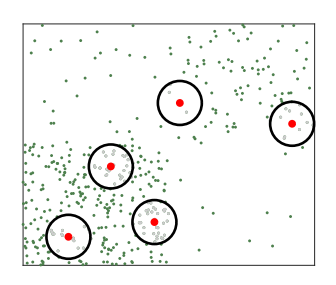
\includegraphics[width=6cm]{img/tesis/PDS.png}
    \caption{Sampling de un PDS en dos dimensiones. Cada elemento muestreado crea un área de rechazo para los siguientes ejemplos (Zhang et al. 2018).}
    \label{fig:PDS}
\end{figure}

\vspace{0.2cm}

El algoritmo que permite samplear de un \textit{Poisson Disk Sampling} (PDS) es el siguiente 

\begin{algorithm}
\caption{Muestreo de un PDS $O(k^2)$, $k$ tamaño de la muestra (Zhang et al. 2018)}\label{alg:alg3}
\begin{algorithmic}
\Require Distancia mínima $r$, conjunto de ejemplos $\{x_i\}_{i=0}^N$

\State $Y \gets \{ x_0 \}$ Uniformemente seleccionado de $\{x_i\}_{i=0}^N$
\State $L \gets \{ 0 \}$
\While{$|L| > 0$}
\State Escoger $i$ de $L$ uniformemente
\State $J \gets$ Hasta $(k - |Y|)$ puntos sampleados uniformemente en el anillo de radio $[r,2r]$ alrededor de $x_i$
\For{$x_j \in J$}
\If{$x_j$ está a distancia mayor a $r$ de todos los elementos en $Y$}
\State $Y \gets Y \cup \{ x_j \}$
\State $L \gets L \cup \{ j \} $
\EndIf
\EndFor
\If{Ningún elemento se agregó a $L$}
\State $L \gets L - {i}$
\EndIf
\EndWhile  
\State \textbf{Output: } $Y$
\end{algorithmic}
\end{algorithm}

La idea es samplear ``hacia afuera'' partiendo desde un punto inicial $x_0$ e iterando el proceso con cada punto nuevo agregado hasta alcanzar la cantidad requerida de sampleos $k$ (notar la importancia de la inicialización en este caso). 


\section{Redes Neuronales}

Una red neuronal artificial es un modelo de aprendizaje de máquinas inspirado en el funcionamiento de las neuronas biológicas que constituyen los cerebros de los animales. \cite{fitch1944warren}

\begin{figure}[ht]
    \centering
    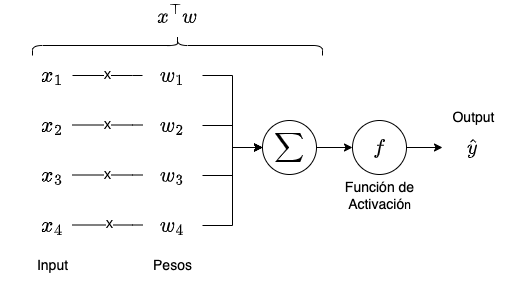
\includegraphics[width=10cm]{img/tesis/perceptron.png}
    \caption{Representación del Perceptrón para un input $x \in \mathbb{R}^4$ y pesos $w \in \mathbb{R}^4$.  }
    \label{fig:perceptron}
\end{figure}

\vspace{0.2cm}

La unidad fundamental de una red neuronal es el Perceptrón (Figura \ref{fig:perceptron}), que es simplemente una función matemática que se encarga de tomar un \textit{input} $x = (x_1 , \dots , x_n) \in \mathbb{R}^n$  y multiplicarlo con un vector de pesos $w = (w_1 , \dots , w_n) \in \mathbb{R}^n$ mediante

\[
\hat{y} = f(x^{\top}w) , 
\]
donde $f: \mathbb{R} \rightarrow \mathbb{R}$ es una función usualmente no lineal conocida como función de activación e $\hat{y} \in \mathbb{R}$ es la salida (\textit{output}).  

\vspace{0.2cm}

Los modelos más comunes de redes neuronales se conocen como \textit{feedforward neural networks} (FFNN) o \textit{multilayer perceptrons} (MLPs) y están compuestos por múltiples perceptrones interconectados en una estructura de capas como lo muestra la Figura \ref{fig:MLPs}.

\begin{figure}[ht]
    \centering
    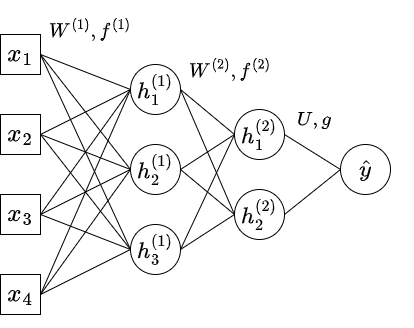
\includegraphics[width=7cm]{img/tesis/MLPs.png}
    \caption{MLP con 2 capas ocultas de pesos $W^{(i)}$ y funciones de activación $f^{(i)}$. Además, incluye una capa de output con función de activación $g$ y pesos $U$. No se agrega un vector de \textit{bias}. }
    \label{fig:MLPs}
\end{figure}

El \textit{output} de cada capa $h^{(k)} = (h^{(k)}_1 , h^{(k)}_2 , \dots , h^{(k)}_{w(k)})$ con $w(k)$ el ancho (cantidad de neuronas) de la capa $k$, se puede describir mediante 
\[
h^{(k)} = f^{(k)}(h^{(k-1)}W^{(k)}  + b^{(k)} ), \quad \forall k \in \{ 1 , \dots , l \} , \quad h^{(0)} = x ,   
\]
donde $l$ es la profundidad de la red, $W$ la matriz de pesos y $b$ el vector de \textit{bias}. La última capa, encargada de producir el \textit{output} de la red, se obtiene de 
\[
\hat{y} = g(h^{(l)}U + c ) , 
\]
donde $c$ es un vector de bias, $U$ una matriz de pesos y $g$ es la función aplicada en la capa de \textit{output} que cambia según el tipo de problema que se quiera resolver, ya sea de clasificación o regresión. 

\subsection{Descenso del Gradiente Estocástico} 

\subsubsection{Introducción }

El aprendizaje de una red neuronal se realiza en base a la actualización de las matrices de peso $W^{(k)}$ y los \textit{bias} $b^{(k)}$ con el objetivo de minimizar el valor de la función de error (\textit{loss}) $l(\hat{y},y)$ que depende de la predicción de la red neuronal $\hat{y}$ y la etiqueta (o valor) real del dato $y$. 

\vspace{0.2cm}

Entre los algoritmos utilizados para la minimización de la función de error $l(\hat{y},y)$ se pueden distinguir 
\begin{itemize}
    \item Métodos Batch o Determinísticos: Son aquellos que utilizan el conjunto de entrenamiento completo en cada iteración y tienden a quedar atrapados en óptimos locales. 
    
    \item Métodos Estocásticos (\textit{Online}): Aquellos que utilizan un solo ejemplo a la vez para el entrenamiento y que resultan ineficientes para grandes volúmenes de datos. 
    
    \item Métodos \textit{Minibatch} Estocásticos: Aquellos que utilizan un subconjunto reducido de ejemplos y promedian los gradientes para obtener el valor esperado.
    
\end{itemize}

\begin{figure}[ht]
    \centering
    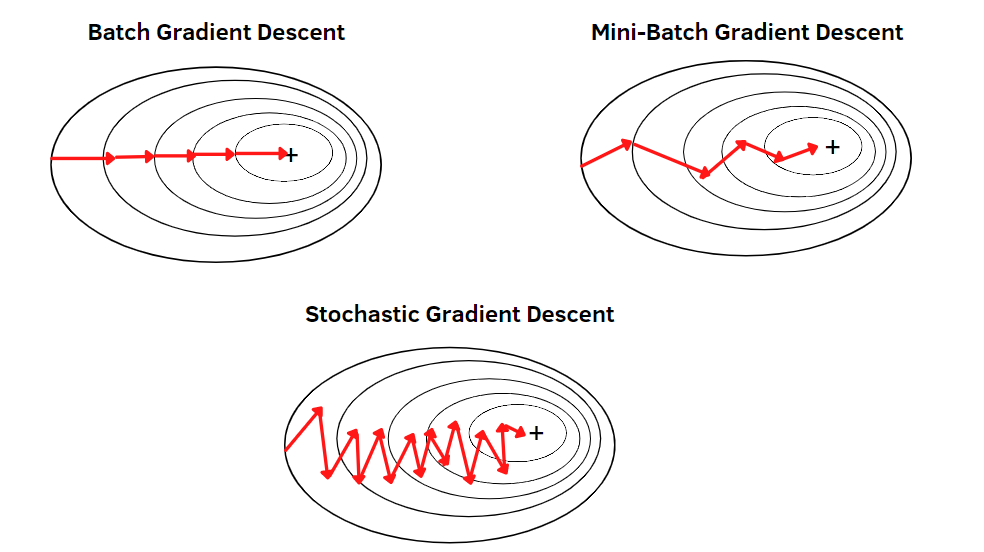
\includegraphics[width=9cm]{img/tesis/SGD.png}
    \caption{Representación de distintos tipos de descensos del gradiente según el tamaño del \textit{Batch} (Wash 2022) \cite{GradientDescent}.}
    \label{fig:SGD}
\end{figure}

Nos centraremos en este último pues es uno de los más utilizados para el entrenamiento de redes neuronales debido a su rapidez y capacidad de convergencia superior a otros métodos \cite{WILSON20031429}, \cite{article}.

\vspace{0.2cm}

De manera formal, sea $\theta$ el parámetro que se busca encontrar y $J^{*}(\theta)$ la función objetivo que depende de la medida de desempeño $l(\hat{y},y) = l(f(x , \theta),y) $ según: 
\[
J^{*}(\theta) = \mathbb{E}_{(x,y) \sim p_{\text{data}}} l(f(x , \theta),y) .
\]
El objetivo es minimizar el error esperado sobre la distribución generada de los datos $p_{\text{data}}$. Para realizar esta tarea, reemplazaremos la expresión $J^{*}$ por la aproximación 
\[
J(\theta) = \mathbb{E}_{(x,y) \sim \hat{p}_{\text{data}}} l(f(x , \theta),y) = \frac{1}{k}\sum_{i=1}^{k}l(f(x_i , \theta),y_i) , 
\]
es decir, el promedio de los errores para un \textit{batch} de tamaño $k$. Notar que en esta segunda expresión, los datos fueron generados por una distribución $\hat{p}_{\text{data}}$ a priori distinta de $p_{\text{data}}$. 

\subsubsection{Descenso del Gradiente Estocástico: Mini-Batch}

Con la función a minimizar $J(\theta)$ definida, la actualización de los parámetros $\theta$ se realiza mediante 
\[
\theta_{t+1} = \theta_t - \rho_t \frac{1}{|B|}\sum_{i \in B}\grad l(f(x_i , \theta_t),y_i) , \quad B \sim \mathcal{P} ,  
\]
donde $B \subset \{1 , \dots , N\}$ es el conjunto de índices del \textit{mini-batch} sampleado según $\mathcal{P}$, normalmente de manera uniforme entre todo el conjunto de entrenamiento que no ha sido visto previamente y $\rho_t$ la tasa de aprendizaje (\textit{learning rate}) del algoritmo en el instante $t$. 

\subsubsection{Épocas de Entrenamiento}

En el contexto del \textit{Deep Learning}, las épocas se definen como ciclos de entrenamiento en el que se recorre completamente un conjunto de datos iterando a través de \textit{batchs}. Una mayor cantidad de épocas permite que los modelos aprendan de manera gradual el conjunto sobre el cual se esta entrenando, pero también deben estar acotadas a un número máximo para prevenir el \textit{overfitting} (el sobreajuste no permite generalizar a datos no vistos anteriormente). La elección correcta de las épocas va a depender de la complejidad de los datos, la arquitectura de la red y las características del problema a resolver. 

\subsection{Redes Neuronales Convolucionales}

Las Redes Neuronales Convolucionales (CNN) son un tipo de red neuronal utilizadas principalmente en problemas cuyo \textit{input} son del tipo matricial como series de tiempo, imágenes, videos, entre otros \cite{INDOLIA2018679}. La principal característica de este tipo de redes es que en algunas de sus capas, se utiliza la operación matemática de convolución, definida como 
\[
s(t) = (x * w)(t) = \int x(a)w(t-a)da , 
\]
donde $x$ es el \textit{input} a convolucionar, $w$ es el kernel con parámetros que se busca aprender y el \textit{output} $s(t)$ se conoce como \textit{feature map}. La ventaja de esta arquitectura y de la operación que utiliza en sus capas, es que la red aprende características locales que no dependen de su posición (invariante a traslación) y que además requieren de una menor cantidad de parámetros entrenables y conexiones, por lo que resultan altamente eficientes y robustas al \textit{overfitting}.
 
\subsection{Autoencoders}

Un \textit{Autoencoder} es un tipo de red neuronal que busca replicar en el \textit{output} el \textit{input} entregado. El desafío es que esto se pueda realizar a partir de una representación de menor dimensionalidad que el \textit{input} a través de un cuello de botella en la arquitectura de la red \cite{Zhang2018ABA}.


\begin{figure}[ht]
    \centering
    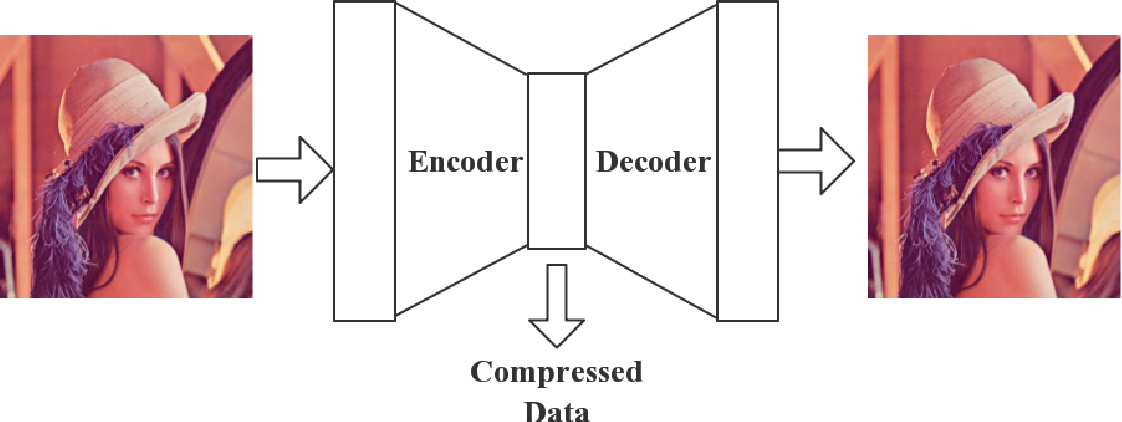
\includegraphics[width=10cm]{img/tesis/autoencoder.png}
    \caption{Autoencoder, el cuello de botella en la mitad de la estructura codifica una representación de menor dimensionalidad del \textit{input} (Zhang 2018).}
    \label{fig:autoencoder}
\end{figure}

El \textit{Autoencoder} en la Figura \ref{fig:autoencoder}) se compone de 2 partes, la primera denominada \textit{encoder}, es la que se encarga de extraer la información más representativa del \textit{input}. La segunda llamada \textit{decoder}, es la que se encarga de recrear la imagen en base a la representación provista. 

\vspace{0.2cm}

Este tipo de red, que si bien su estructura podría ser del tipo FFNN o CNN, no requiere conocer la etiqueta del \textit{input} ($y$), es decir, se enmarca dentro de los métodos de aprendizaje de máquinas no supervisados. 

\subsection{One Shot Learning}

\textit{One Shot Learning} o (\textit{Few Shot Learning}) es un método de aprendizaje de máquinas utilizado comúnmente en el área de visión computacional y que busca reducir drásticamente la cantidad de ejemplos necesarios para clasificar objetos \cite{OMAHONY2019186}.

\vspace{0.2cm}

\begin{figure}[ht]
    \centering
    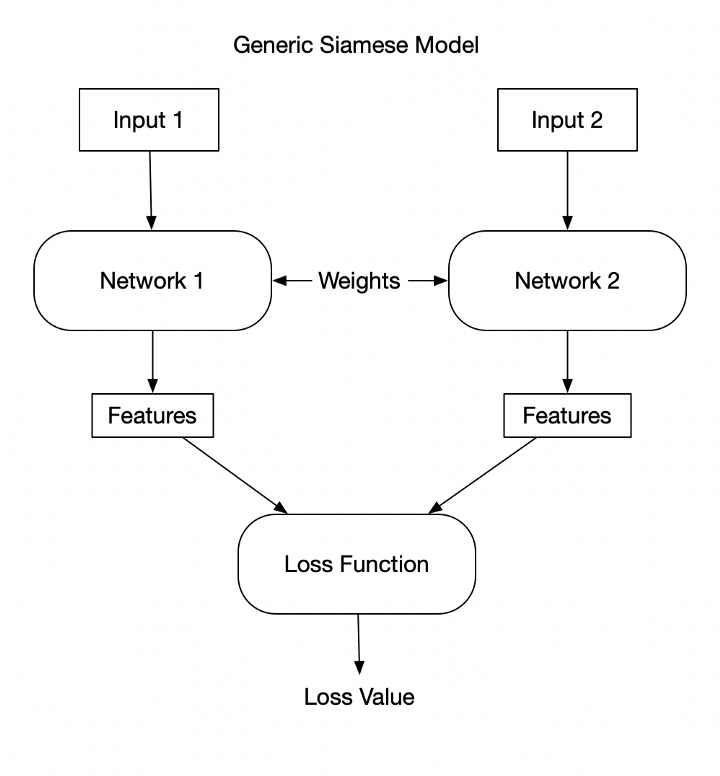
\includegraphics[width=7cm]{img/tesis/siamese.png}
    \caption{Arquitectura One Shot Learning, los \textit{batches} de entrenamiento se componen de tuplas de ejemplos que son entregados en cada sección de la red.}
    \label{fig:oneshot}
\end{figure}


Para lograr esto, se implementa una red del tipo siamés representada en la Figura \ref{fig:oneshot} que consta de 2 CNN entrenadas en paralelo y que comparten los mismos pesos. Además, 2 FFNN también entrenadas en paralelo pero con pesos independientes se encargan de interpretar las características entregadas y su relación. Finalmente, ambas representaciones son comparadas mediante alguna medida de distancia, usualmente euclidiana, para obtener el \textit{score} de similaridad. 

\vspace{0.2cm}

El entrenamiento de este tipo de redes puede ser realizado de múltiples formas entre las que se encuentran: 

\begin{itemize}
    \item \textit{Contrastive Loss}: Esta función de pérdida calculada entre pares de ejemplos busca que datos similares sean mapeados en regiones cercanas del espacio.
    \[
    l(x_i , x_j) = -\log\frac{\exp(d(z_i , z_j)/\tau)}{\sum_{k=1 , k \neq i}^N \exp(d(z_i , z_k)/\tau)} , 
    \]
    Donde $z_i$ y $z_j$ son la representación de los ejemplos $x_i$ y $x_j$ respectivamente. Notar la similitud con una función \textit{Softmax} a la que además se le agrega un factor de normalización (temperatura) $\tau$. La función $d(\cdot, \cdot)$ es alguna métrica de distancia previamente  definida como una distancia coseno o una distancia euclidiana. 
    
    \item \textit{Triplet Loss}: Esta función de pérdida se calcula entre tripletas de ejemplos lo que permite que el entrenamiento se pueda hacer con muy pocos datos. Para cada imagen base, denominada \textit{Anchor}, se escoge una imagen de la misma clase (\textit{Positive}) y una de distinta clase (\textit{Negative}).
    
    \begin{figure}[ht]
    \centering
    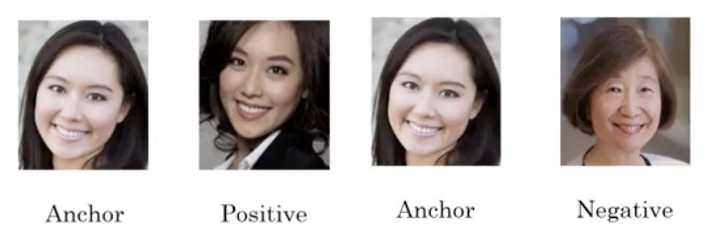
\includegraphics[width=8cm]{img/tesis/triplet_loss.jpeg}
    \caption{Triplet Loss: La imagen \textit{Anchor} se compara con una imagen de misma etiqueta (\textit{Positive}) y una de distinta etiqueta (\textit{Negative}) (Ghandi 2018) \cite{TripletLoss}.}
    \label{fig:triplet_loss}
    \end{figure}
    
    \noindent La función de \textit{triplet loss} tomará en cuenta estas 2 comparaciones según
    \[
    l(x_a , x_p, x_n) = \max(d(z_a, z_p) - d(z_a, z_n) + \text{margin} , 0) , 
    \]
    es decir, considerara la capacidad de la red de reconocer imágenes de igual y distinta clase en simultaneo. 
    
    
\end{itemize}

Ambos métodos tienen la ventaja de que se necesita una pequeña cantidad de datos para aprender a diferenciar, pues, el conjunto de entrenamiento se crea en base a todos los posibles pares (o tríos) de ejemplos que se pueden formar.






